\chapter{PENGUJIAN DAN EVALUASI}
Pada bab ini akan dibahas uji coba dan evaluasi dari sistem yang sudah dibuat. Sistem akan diuji coba fungsionalitasnya dengan menjalankan skenario pengujian fitur-fitur dari sistem yang dibuat. Sistem juga akan diuji coba performa dengan skenario pengujian beban terhadap sistem. Uji coba dilakukan untuk mengevaluasi kinerja dari sistem dengan lingkungan uji coba yang ditentukan.

\section{Lingkungan Uji Coba}
Lingkungan uji coba sistem ini terdiri dari beberapa komponen yaitu \textit{middleware} dan perangkat jaringan yang terhubung. Server yang digunakan sebagai \textit{middleware} merupakan \textit{Virtual Private Server} yang disediakan oleh DPTSI ITS. Perangkat jaringan yang digunakan adalah Cisco Catalyst 3560G. Spesifikasi dari \textit{Middleware} bisa dilihat di tabel \ref{tabelKomponen} 
   \begin{longtable}{|p{0.03\textwidth}|p{0.18\textwidth}|p{0.30\textwidth}|p{0.35\textwidth}|}
   	
   	\caption{Spesifikasi Komponen} \label{tabelKomponen} \\
   	\hline
   	\textbf{No} & \textbf{Komponen} & \textbf{Perangkat Keras} & \textbf{Perangkat Lunak} \\ \hline
   	\endfirsthead
   	
   	\hline
   	\textbf{No} & \textbf{Komponen} & \textbf{Perangkat Keras} & \textbf{Perangkat Lunak} \\ \hline
   	\endhead
   	\endfoot
   	\endlastfoot
   	
   	1 & \textit{Middleware} & 4 Core Processor, 4GB RAM, HDD 64 GB & Ubuntu 18.04.3, MySQL 5.7, Python 3.6, Go1.13.5, Flask 1.0.3, Python 3.6 \\ \hline
   	2 & Switch & 512KB RAM, 38.7 Mpps, 2 Virtual Ethernet interfaces, 28 Gigabit Ethernet interfaces & ios Version 12.2(53)SE2 \\ \hline
   	3 & PC & 8 Core Processor, 8GB RAM, SSD 128 & Ubuntu 18.04, Python 3.6 \\ \hline
		
   	
   \end{longtable}

	\begin{figure}[H]
		\centering
		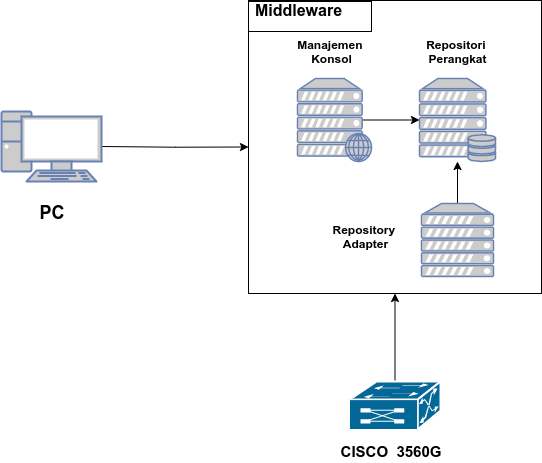
\includegraphics[width=\textwidth]{Images/C-5/Lingkungan-uji-coba.png}
		\caption{Penggunaan storage repositori}
		\label{lingkungan uji coba}
	\end{figure}

\section{Skenario Uji Coba}
Uji coba ini dilakukan untuk menguji fungsionalitas dari sistem yang dibuat telah sesuai dengan perancangan dan sistem benar-benar diimplementasikan dan bekerja sesuai seharusnya. Skenario pengujian dibedakan menjadi 2 bagian yaitu:
\begin{itemize}
	\item \textbf{Uji Fungsionalitas} \\
	Pengujian yang dilakukan berdasarkan fungsionalitas yang disediakan sistem.
	\item \textbf{Uji Performa} \\
	Pengujian yang dilakukan untuk melihat waktu yang diperlukan untuk menyimpan konfigurasi perangkat jaringan.
\end{itemize}  
	
    
    
    \subsection{Skenario Uji Coba Fungsionalitas}
    Uji fungsionalitas dibagi menjadi beberapa bagian antara lain yaitu \textit{user} mengelola repositori, \textit{user} mengirim file konfigurasi, \textit{user} melakukan checkout commit, mengunduh file setelah checkout commit, dan percabangan commit.
    	
    	\subsubsection{Uji Fungsionalitas \textit{User} Mengelola Repositori}
    	Uji coba ini bertujuan untuk memastikan fitur dari mengelola repositori dapat dijalankan dengan benar.
    	Uji coba dilakukan dengan user mengakses sistem melalui rute untuk mengelola repositori. \textit{User} mengirimkan request ke manajemen konsol. Rancangan pengujian dan hasil yang diinginkan dapat dilihat pada Tabel .
    	\begin{longtable}{|p{0.03\textwidth}|p{0.23\textwidth}|p{0.27 \textwidth}|p{0.33\textwidth}|}
    		
    		\caption{skenario uji fungsionalitas user mengelola repositori} \label{mengelolaRepositori} \\
    		\hline
    		\textbf{No} & \textbf{Rute} & \textbf{Uji Coba} & \textbf{Harapan} \\ \hline
    		\endfirsthead
    		
    		\hline
    		\textbf{No} & \textbf{Rute} & \textbf{Uji Coba} & \textbf{Harapan} \\ \hline
    		\endhead
    		\endfoot
    		\endlastfoot
    		
    		1 & \path{/home} & Mengirimkan request Get menuju manajemen konsol & Request berhasil diterima manajemen konsol, kemudian manajemen konsol meampilkan halaman daftar perangkat yang dihubungkan dan menampilkan form untuk menambahkan perangkat. \\ \hline
    		2 & \path{/home} & Mengirimkan request Post menuju manajemen konsol & Request berhasil diterima manajemen konsol, kemudian manajemen konsol membuat repositori untuk perangkat yang ditambahkan.\\ \hline
    		3 & \path{/{reponame}/branch/{branchname}} & Mengirimkan request menuju manajemen konsol & Request berhasil diterima manajemen konsol, kemudian manajemen konsol menampilkan daftar commit pada repositori. \\ \hline 
    		4 & \path{/{username}/{reponame}/commit/{hashcommit}} & Mengirimkan request menuju manajemen konsol & Request berhasil diterima manajemen konsol, kemudian manajemen konsol menampilkan diff commit dari hash yang dipilih dengan \textit{commit parent}-nya. \\ \hline
    		5 & \path{/delete/{reponame}} & Mengirimkan request menuju manajemen konsol & Request berhasil diterima manajemen konsol, kemudian sistem menghapus repositori.\\ \hline
	    \end{longtable}
    	\subsubsection{Uji Fungsionalitas User Mengirim Konfigurasi}
    	Uji coba ini bertujuan untuk memastikan perangkat jaringan dapat mengirim file konfigurasi ke dalam repositori sistem. Juga untuk memastikan setiap ada perubahan pada konfigurasi perangkat maka sistem otomatis melakukan commit pada git repositori.\\
    	\indent Uji coba ini dilakukan dengan cara user mengirimkan file konfigurasi dari perangkat jaringan menuju \textit{middleware} sistem. Pengiriman konfigurasi menggunakan protokol yang didukung oleh perangkat jaringan. Setelah file dikirim, \textit{middleware} akan melihat ada perubahan dalam repositori sehingga \textit{middleware} langsung menjalankan perintah commit dan push. Setelah commit dilakukan dapat dilihat histori commit dari repositori.\\
    	\indent Uji coba berhasil ketika file konfigurasi berhasil terkirim dan pada repositori terbuat commit baru.
    	
    	\subsubsection{Uji Fungsionalitas \textit{User} Merubah Versi}
    	Uji coba ini bertujuan untuk memastikan admin dapat merubah versi commit dari file konfigurasi di dalam repositori.\\
    	\indent Uji coba ini dilakukan dengan cara user me-klik tombol pilih versi pada daftar commit di dalam repositori. Sistem akan melakukan checkout commit pada repositori lokal sehingga versi konfigurasi berubah sesuai versi yang dipilih. Uji coba perubahan versi dilakukan pada \textit{branch} yang sama dan \textit{branch} yang berbeda.\\
    	\indent Uji coba berhasil ketika versi dari file konfigurasi berhasil berubah sesuai dengan yang diinginkan.
    	
    	\subsubsection{Uji Fungsionalitas Unduh Konfigurasi}
    	Uji coba ini bertujuan untuk memastikan perangkat jaringan dapat mengunduh file konfigurasi dari \textit{middleware} sistem. Uji coba juga untuk memastikan perangkat jaringan bisa mengunduh semua versi yang ada di \textit{middleware} sistem. \\
    	\indent Uji coba ini dilakukan dengan cara user mengakses perangkat jaringan yang terhubung dengan \textit{Middleware}. User kemudian mengunduh file konfigurasi dari \textit{middleware} kedalam perangkat jaringan. File konfigurasi diunduh sebelum versi dirubah dan setelah versi dirubah. \\
    	\indent Uji coba berhasil ketika perangkat jaringan bisa mengunduh file konfigurasi dari \textit{middleware} sistem.
    	
    	\subsubsection{Uji Fungsionalitas Percabangan Commit}
    	Uji coba ini bertujuan untuk memastikan ketika perangkat jaringan mengirim konfigurasi dan kondisi versi bukan merupakan versi terbaru maka akan terbentuk cabang baru pada commit repositori.\\
    	\indent Uji coba ini dilakukan dengan cara user melakukan checkout pada repositori. Setelah checkout, user kemudian mengakses perangkat jaringan dan mengirimkan file konfigurasi ke \textit{middleware}. Karena posisi head tidak berada pada posisi commit terbaru maka sistem akan otomatis membuat cabang baru setelah ada perubahan di dalam repositori.\\
    	\indent Uji coba berhasil ketika setelah pengiriman file konfigurasi, repositori perangkat otomatis membuat cabang baru.
    	 
    \subsection{Skenario Uji Coba Performa}
    	Uji performa digunakan untuk menguji bagaimana ketahanan sistem dalam menyimpan konfigurasi perangkat jaringan dan mengatur versi perangkat jaringan.\\
    	\indent Uji performa dilakukan dengan cara mengirim konfigurasi dari perangkat jaringan menuju middlware sistem secara bertahap. Perubahan yang dilakukan pada konfigurasi dilakukakan secara bertahap mulai dari 50 perubahan hingga 500 perubahan dengan penambahan 50 perubahan di setiap tahap. Uji coba dilakukan untuk melihat beberapa storage yang digunakan oleh repositori untuk penyimpanan konfigurasi dan dalam menyimpan perubahan. Uji coba juga dilakukan untuk melihat waktu yang diperlukan untuk merubah versi konfigurasi.\\ 
    	\indent Hasil yang diharapkan dari pengujian ini adalah sistem memiliki \textit{storage} yang cukup untuk menyimpan konfigurasi minimal selama satu tahun. 
    
\section{Hasil Uji Coba dan Evaluasi}
	Berikut ini dijelaskan hasil coba dan evaluasi berdasarkan skenario yang sudah dijelaskan pada subbab sebelumnya.
	
	\subsection{Uji Fungsionalitas}
	Berikut ini dijelaskan hasil dari pengujian fungsionalitas pada sistem yang sudah dibangun.
	
	\subsubsection{Uji Fungsionalitas User Mengelola Repositori}
	Uji coba dilakukan dengan mengakses manajemen konsol melalui rute yang ditentukan pada tabel \ref{hasilmengelolaRepositori}. Hasil pengujian dapat dilihat pada tabel .
	\begin{longtable}{|p{0.03\textwidth}|p{0.23\textwidth}|p{0.40 \textwidth}|p{0.10\textwidth}|}
		
		\caption{Hasil uji fungsionalitas user mengelola repositori} \label{hasilmengelolaRepositori} \\
		\hline
		\textbf{No} & \textbf{Rute} & \textbf{Harapan} & \textbf{Hasil} \\ \hline
		\endfirsthead
		
		\hline
		\textbf{No} & \textbf{Rute} & \textbf{Harapan} & \textbf{Hasil} \\ \hline
		\endhead
		\endfoot
		\endlastfoot
		1 & \path{/home} & Request berhasil diterima manajemen konsol, kemudian manajemen konsol meampilkan halaman daftar perangkat yang dihubungkan dan menampilkan form untuk menambahkan perangkat. & OK \\ \hline
		2 & \path{/home} & Request berhasil diterima manajemen konsol, kemudian manajemen konsol membuat repositori untuk perangkat yang ditambahkan. & OK\\ \hline
		3 & \path{/{reponame}/branch/{branchname}} & Request berhasil diterima manajemen konsol, kemudian manajemen konsol menampilkan daftar commit pada repositori. & OK \\ \hline 
		4 & \path{/{username}/{reponame}/commit/{hashcommit}} & Request berhasil diterima manajemen konsol, kemudian manajemen konsol menampilkan diff commit dari hash yang dipilih dengan \textit{commit parent}-nya. & OK \\ \hline
		5 & \path{/delete/{reponame}} & Request berhasil diterima manajemen konsol, kemudian sistem menghapus repositori. & OK\\ \hline
	
	\end{longtable}

	\subsubsection{Uji Fungsionalitas User Mengirim Konfigurasi}
    Uji coba ini dilakukan dengan cara user mengirim file konfigurasi dari perangkat jaringan menggunakan protokol TFTP, FTP, dan SCP. Keterangan hasil uji bisa dilihat pada tabel.
    \begin{longtable}{|p{0.03\textwidth}|p{0.23\textwidth}|p{0.40\textwidth}|p{0.10\textwidth}|}
    	
    	\caption{Hasil uji fungsionalitas user mengelola repositori} \label{hasilmengelolaRepositori} \\
    	\hline
    	\textbf{No} & \textbf{Protokol} & \textbf{Harapan} & \textbf{Hasil} \\ \hline
    	\endfirsthead
    	
    	\hline
    	\textbf{No} & \textbf{Protokol} & \textbf{Harapan} & \textbf{Hasil} \\ \hline
    	\endhead
    	\endfoot
    	\endlastfoot
    	1 & TFTP & File Konfigurasi terbuat di dalam repositori & OK\\ \hline
    	2 & FTP & File Konfigurasi terbuat di dalam repositori & OK\\ \hline
    	3 & SCP & File Konfigurasi terbuat di dalam repositori & OK\\ \hline
    	
    \end{longtable}

	\subsubsection{Uji Fungsionalitas \textit{User} Merubah Versi}
	Uji coba ini dilakukan dengan cara user me-klik tombol pilih versi pada commit yang diinginkan. Keterangan hasil uji bisa dilihat pada tabel \ref{hasilCheckoutCommit}.
	\begin{longtable}{|p{0.03\textwidth}|p{0.36\textwidth}|p{0.45\textwidth}|p{0.10\textwidth}|}
		
		\caption{Hasil uji fungsionalitas user checkout commit} \label{hasilCheckoutCommit} \\
		\hline
		\textbf{No} & \textbf{Perubahan} & \textbf{Harapan} & \textbf{Hasil} \\ \hline
		\endfirsthead
		\hline
		\textbf{No} & \textbf{Perubahan} & \textbf{Harapan} & \textbf{Hasil} \\ \hline
		\endhead
		\endfoot
		\endlastfoot
		1 & Perubahan pada satu branch & Versi pada repositori berubah & OK\\ \hline
		2 & Perubahan pada branch berbeda & Versi pada repositori berubah & OK\\ \hline
		
	\end{longtable}

	\subsubsection{Uji Fungsionalitas Unduh Konfigurasi}
	Uji coba dilakukan dengan cara administrator membuka perangkat jaringan dan mengunduh konfigurasi dari sistem. Keterangan hasil uji bisa dilihat pada tabel \ref{hasilUnduhKonfig}.
	\begin{longtable}{|p{0.03\textwidth}|p{0.30\textwidth}|p{0.50\textwidth}|p{0.10\textwidth}|}
		
		\caption{Hasil uji fungsionalitas user checkout commit} \label{hasilUnduhKonfig} \\
		\hline
		\textbf{No} & \textbf{Unduhan} & \textbf{Harapan} & \textbf{Hasil} \\ \hline
		\endfirsthead
		\hline
		\textbf{No} & \textbf{Unduhan} & \textbf{Harapan} & \textbf{Hasil} \\ \hline
		\endhead
		\endfoot
		\endlastfoot
		1 & Sebelum checkout & File konfigurasi berhasil diunduh & OK\\ \hline
		2 & Setelah checkout & File konfigurasi berhasil diunduh & OK\\ \hline
		
	\end{longtable}
	
	
	\subsubsection{Uji Fungsionalitas Percabangan Commit}
	Uji coba ini dilakukan dengan cara mengunggah konfigurasi perangkat menuju sistem dengan kondisi versi dalam sistem bukan versi terbaru yang dicatat. Keterangan hasil ujicoba bisa dilihat pada tabel.
	
	\begin{longtable}{|p{0.03\textwidth}|p{0.30\textwidth}|p{0.45\textwidth}|p{0.10\textwidth}|}
		
		\caption{Hasil uji fungsionalitas percabangan commit} \label{hasil precabangan commit} \\
		\hline
		\textbf{No} & \textbf{Urutan Cabang} & \textbf{Harapan} & \textbf{Hasil} \\ \hline
		\endfirsthead
		\hline
		\textbf{No} & \textbf{Urutan Cabang} & \textbf{Harapan} & \textbf{Hasil} \\ \hline
		\endhead
		\endfoot
		\endlastfoot
		1 & 1 & Cabang terbuat & OK\\ \hline
		2 & 2 & Cabang terbuat & OK\\ \hline
		3 & 3 & Cabang terbuat & OK\\ \hline
	\end{longtable}
	
   	
    \subsection{Hasil Uji Performa}
    Uji performa dilakukan pada \textit{middleware} sistem. Pengujian dilakukan dengan mengirimkan konfigurasi dari perangkat jaringan menuju \textit{middleware}. Jumlah perubahan dimulai dari 50 perubahan sampe 500 perubahan dan ditambahkan secara bertahap dengan interval 50 perubahan. Hasil uji coba setelah dilakukan perubahan konfigurasi dari perangkat jaringan dan disimpan di \textit{middleware} dapat dilihat pada Gambar\ref{ukuranRepo}. Rata-rata storage yang digunakan untuk setiap perubahan dapat dilihat pada Gambar\ref{Rata-rataperubahan}. Dalam uji performa uga dilakukan pengujian untuk melihat response time ketika melakukan checkout (pemindahan versi) di dalam repositori. Hasil pengujian response time dapat dilihat pada grafik \ref{response time checkout}.
    	
    	\begin{figure}[H]
    	\centering
    	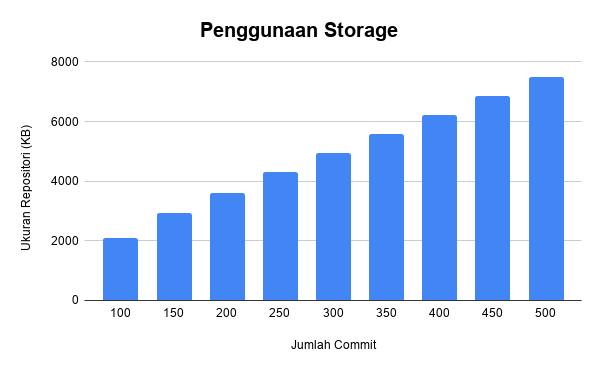
\includegraphics[width=\textwidth]{Images/C-5/Penggunaan-Storage.png}
    	\caption{Penggunaan storage repositori}
    	\label{ukuranRepo}
    	\end{figure}
    
    	\begin{figure}[H]
	    	\centering
	    	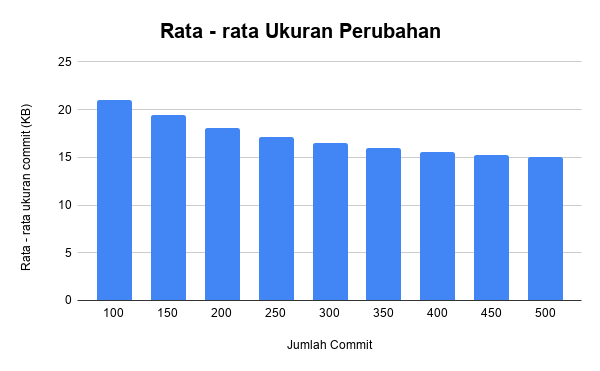
\includegraphics[width=\textwidth]{Images/C-5/Rata-rata-Ukuran-Perubahan.png}
	    	\caption{Penggunaan storage repositori}
	    	\label{Rata-rataperubahan}
	    \end{figure}
    
    \begin{figure}[H]
    	\centering
    	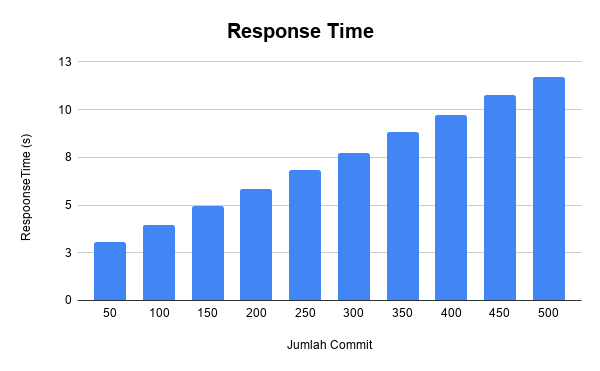
\includegraphics[width=\textwidth]{Images/C-5/Response-Time.png}
    	\caption{Penggunaan storage repositori}
    	\label{response time checkout}
    \end{figure}
    
    \indent Dari grafik \ref{ukuranRepo} dapat dilihat bahwa penggunaan storage tidak mengalami perbedaan yang banyak. Dapat dilihat bahwa storage yang digunakan berubah linier terhadap jumlah commit (perubahan) yang dilakukan. Jika diasumsikan dalam setahun dilakukan perubahan setiap hari pada perangkat jaringan maka minimal storage yang dibutuhkan untuk mencatat perubahan satu perangkat adalah 6 MB.\\
    \indent Dari grafik \ref{Rata-rataperubahan} dapat dilihat bahwa rata-rata storage yang dibutuhkan untuk menyimpan perubahan semakin sedikit ketika jumlah perubahan semakin banyak. Dari uji coba yang dilakukan ukuran perubahan konfigurasi yang disimpan di dalam repositori adalah 15-25 KB.\\
    \indent Dari grafik \ref{response time checkout} dapat dilihat bahwa jumlah  perubahan yang yang dicatat mempengaruhi waktu yang diperlukan untuk melakukan checkout commit. Semakin banyak perubahan yang disimpan di dalam repositori maka waktu yang diperlukan untuk melakukan checkout (pemindahan versi) akan semakin lama. Hal ini terjadi karena semakin banyak perubahan yang dicatat maka semakin banyak juga data perubahan yang diambil untuk ditampilkan.
     
    	